\documentclass[11pt]{amsart}
\usepackage[
style=apa, natbib=true,
]{biblatex}
\addbibresource{biblio.bib} 
%prepared in AMSLaTeX, under LaTeX2e
\addtolength{\oddsidemargin}{-.65in}
\addtolength{\evensidemargin}{-.65in}
\addtolength{\topmargin}{-.5in}
\addtolength{\textwidth}{1.2in}
\addtolength{\textheight}{1.0in}
\renewcommand{\baselinestretch}{1.06}

\usepackage{wrapfig,fancyvrb,xspace}
\usepackage{palatino,bm,stmaryrd}
\usepackage[final]{graphicx}
\usepackage[pdftex, colorlinks=true, plainpages=false, linkcolor=blue, citecolor=red, urlcolor=blue]{hyperref}

% macros
\newcommand{\bn}{\mathbf{n}}
\newcommand{\bq}{\mathbf{q}}
\newcommand{\bu}{\mathbf{u}}
\newcommand{\bv}{\mathbf{v}}
\newcommand{\bw}{\mathbf{w}}
\newcommand{\bx}{\mathbf{x}}

\newcommand{\bX}{\mathbf{X}}

\newcommand{\bsigma}{\bm{\sigma}}
\newcommand{\bomega}{\bm{\omega}}

\newcommand{\cH}{\mathcal{H}}
\newcommand{\cK}{\mathcal{K}}
\newcommand{\cT}{\mathcal{T}}
\newcommand{\cV}{\mathcal{V}}

\newcommand{\dx}{\mathrm{dx}}
\newcommand{\ds}{\mathrm{ds}}

\newcommand{\RR}{\mathbb{R}}

\newcommand{\Div}{\nabla\cdot}
\newcommand{\eps}{\epsilon}
\newcommand{\grad}{\nabla}
\newcommand{\lam}{\lambda}

\newcommand{\jump}[1]{\llbracket #1 \rrbracket }


\title{Gas in a porous media, using Firedrake}
\author{Tara Shreve}
\author{Ed Bueler}
\date{\today}

\begin{document}
\maketitle
%\begin{abstract}
%FIXME
%\end{abstract}

\thispagestyle{empty}

\section{A porous medium model for Darcy-type gas flow}

Suppose $\Omega$ is a 2D or 3D domain with well-behaved boundary, such as a rectangle or other polygon in 2D, or a polyhedron in 3D.  We will use $x,y$ for the horizontal coordinates and $z$ for the vertical coordinate.  (In 2D we use only $x,z$.)  Note $z$ is measured positive upward.

Within $\Omega$ we assume there is a matrix of porous material with spatially-variable porosity $\phi(x,y,z)$ and permeability $k(x,y,z)$; these are assumed independent of time.  An ideal gas flows through the medium, and we will take the properties of this gas to be positive constants: $R$ is the gas constant, $T$ is the absolute temperature, and $M$ is the molar mass.  The ideal gas law says the density $\rho$ and pressure $P$ are proportional via $c = RT/M$, a positive constant:
\begin{equation}
c \rho = P.  \label{eq:ideal}
\end{equation}

We assume that the gas flow satisfies Darcy's law \citep{Fowler2011}, thus the volumetric flux $\bq$ is driven by the gradient of the deviation of the gas pressure from the (litho)static pressure distribution $P_0(z)$:
\begin{equation}
\bq = - \frac{k}{\mu} \grad\left(P - P_0\right) \label{eq:pmtime:darcy}
\end{equation}
Here $\mu$ is the dynamic viscosity of the gas, again taken to be constant, and note that a formula for $P_0(z)$ is derived momentarily.  Because mass is conserved, additionally we have:
\begin{equation}
\phi \frac{\partial \rho}{\partial t} + \Div \left(\rho\, \bq\right) = 0. \label{eq:pmtime:masscont}
\end{equation}
Here we are assuming no mass sources or sinks, as otherwise there would be an additional function on the right side.

Certain observations regarding these equations should be made.  First, gas density must be non-negative: $\rho\ge 0$.  Second, relative to the classic mass continuity statement ``$\partial\rho/\partial t + \Div(\rho \bv)=0$'' \citep[for example]{Tadmor2012}, where $\bv$ is the fluid velocity, note that \eqref{eq:pmtime:masscont} is scaled with the (dimensionless) porosity $\phi$.  However, $\phi$ is also implicit in the definition of $\bq$ because it is the gas volume per unit area of any face of the porous matrix: $\bq = \phi \bv$.  While the velocity $\bv$ may be helpful in understanding the solution, it is not required when stating the model.

\newcommand{\Patm}{P_{\text{atm}}}
The lithostatic distribution $P_0$ is the pressure field for a mass (gas) distribution for which there is no flow.  Considering a fully-connected porous medium with stationary gas, because of gravity the mass of gas in each layer contributes to the pressure on the gas below, that is, $dP_0 = - g \rho_0\,dz = - (g/c) P_0\,dz$ where $g>0$ is the acceleration of gravity.  If we assume that the top of the porous medium, at height $z=L$, is at atmospheric pressure $\Patm$ then we have the following formula:
\begin{equation}
P_0(z) = \Patm e^{g(L-z)/c}. \label{eq:staticpressure}
\end{equation}
Clearly, $P_0$ is independent of the solution pressure $P$, and (also clearly) substitution of $P_0$ for $P$ in \eqref{eq:pmtime:darcy} gives $\bq=0$, that is, no flow.

Regarding units of the solution variables in the above equations, $\rho(t,x,y,z)$ is in SI units of $\text{kg}\,\text{m}^{-3}$, $P(t,x,y,z)$ in $\text{Pa} = \text{N}\,\text{m}^{-2}$, and $\bq(t,x,y,z)$ in $\text{m}^3\,\text{m}^{-2}\,\text{s}^{-1} = \text{m}\,\text{s}^{-1}$.  Also the porosity $\phi$ is a dimensionless ratio of volumes, thus $0\le \phi \le 1$, the permeability $k$ is in $\text{m}^2$, the constant $c$ is in $\text{J}\,\text{kg}^{-1}$, and the dynamic viscosity $\mu$ is in $\text{Pa}\,\text{s}$.

Considering the system of equations \eqref{eq:ideal}--\eqref{eq:staticpressure}, it is straightforward to eliminate the pressure $P$ and flux $\bq$, if this is desired:
\begin{equation}
\phi \frac{\partial \rho}{\partial t} - \Div \left(\frac{k}{\mu} \rho \grad\left(c \rho - P_0\right)\right) = 0. \label{eq:pmtime:primal}
\end{equation}
This form is comparable to the better-known heat equation
\begin{equation}
\frac{\partial u}{\partial t} - \Div(\grad u) = 0. \qquad \text{\emph{(heat equation)}}\label{eq:heattime:primal}
\end{equation}
An important property of \eqref{eq:heattime:primal} is that the operator $\Div \grad = \grad^2$ acts as an invertible matrix when finding the solution $u$.  However, since $\rho$ appears as a flux coefficient in \eqref{eq:pmtime:primal}, invertibility is lost in \eqref{eq:pmtime:primal} if $\rho\to 0$ somewhere.  Such ``degeneration'' of the diffusivity is a well-known concern with the porous medium equation \eqref{eq:pmtime:primal} \citep[for example]{Vazquez2007}, and it will influence the numerical solution method below.

The model above is time dependent, but setting $\partial \rho/\partial t = 0$ yields the steady-state version.  First, for \eqref{eq:pmtime:masscont} we define the (conserved) mass flux
\begin{equation}
\bsigma = \rho \bq, \label{eq:massflux}
\end{equation}
with units of $\text{kg}\,\text{m}^{-2}\,\text{s}^{-1}$.  The steady-state model is now written in terms of the conserved mass density $\rho$ and its flux $\bsigma$:
\begin{subequations}
\label{eq:pm:strong}
\begin{align}
\bsigma &= - \frac{k}{\mu} \rho \grad\left(c \rho - P_0\right) \label{eq:darcy} \\
\Div \bsigma &= 0 \label{eq:masscont}
\end{align}
\end{subequations}

Suitable boundary conditions must apply to system \eqref{eq:pm:strong}.  On the ``Dirichlet'' part of the boundary, denoted $\Gamma_D \subset \partial\Omega$, the density is given by a continuous function $\rho_D(x,y,z)$.  Equivalently the pressure may be given on $\Gamma_D$.  On the remainder of the boundary $\Gamma_N = \partial\Omega \setminus \Gamma_D$, the ``Neumann'' boundary, the normal mass flux is zero:
\begin{subequations}
\label{eq:strongbcs}
\begin{align}
\rho|_{\Gamma_D}               &= \rho_D \\
(\bsigma\cdot \bn)|_{\Gamma_N} &= 0
\end{align}
\end{subequations}
It is straightforward to extend the model with provided values of the mass flux, i.e.~$(\bsigma\cdot \bn)|_{\Gamma_N}= \sigma_N$ where $\sigma_N$ is given, for a non-homogeneous Neumann condition.  System \eqref{eq:pm:strong} with boundary conditions \eqref{eq:strongbcs} apparently forms a well-posed problem as long as $\Gamma_D$ has positive measure (within $\partial\Omega$) and $\rho_D\ge 0$.  In the time-dependent case, classical solutions exist if additionally $\rho_D$ is actually positive and the initial density is positive \citep[Theorem 3.1]{Vazquez2007}.

The equations above form a nonlinear model for the density $\rho$, with degeneration of the diffusivity if $\rho \to 0$.  However, a straightforward substitution allows us to rewrite the problem as a semi-linear\footnote{``Semi-linear'' means that the highest-order term is linear \citep[section 1.1]{Evans2010}.} system, essentially as a linear diffusion problem along with (nonlinear) advection from the lithostatic pressure $P_0$.  Let
\begin{equation}
u = \rho^2 \label{eq:pm:defu}
\end{equation}
and define convenience constants
\begin{equation}
\alpha = \frac{c}{2\mu}, \quad \beta = \frac{1}{\mu}. \label{eq:pm:convenience}
\end{equation}
Then \eqref{eq:pm:strong}, \eqref{eq:strongbcs} becomes
\begin{subequations}
\label{eq:pm:strongu}
\begin{align}
\bsigma &= - \alpha k \grad u + \beta k \sqrt{u}\, \grad P_0 & &\text{on } \Omega \label{eq:pm:strongu:darcy} \\
\Div \bsigma &= 0 & & \label{eq:pm:strongu:masscont} \\
u &= \rho_D^2 & &\text{on } \Gamma_D  \label{eq:pm:strongu:bcD} \\
\bsigma\cdot \bn &= 0 & &\text{on } \Gamma_N  \label{eq:pm:strongu:bcN} 
\end{align}
\end{subequations}
The (mixed) strong-form system \eqref{eq:pm:strongu} is a steady-state, semi-linear advection-diffusion problem, for the solution pair $(\bsigma,u)$, in which $\grad P_0$ acts as a kind of transport velocity.  Eliminating $\bsigma$ is also straightforward, yielding primal form
\begin{equation}
-\alpha \Div(k\grad u) + \beta \Div(k \sqrt{u}\, \grad P_0) = 0. \label{eq:pm:primalstrongu}
\end{equation}
In either form, the density $\rho$ and pressure $P$ are easily recovered via \eqref{eq:pm:defu}, \eqref{eq:ideal} as long as the solution satisfies $u\ge 0$.

\section{Mixed weak form (with discontinuous permeability)}

We will solve system \eqref{eq:pm:strongu} by a conservative mixed finite element (FE) method \citep{Boffi2013}.  In this section we derive the weak form, needed for an FE method, via an element-wise weak form.  This derivation allows the permeability field to be discontinuous across element edges, and it makes the conservation property of the FE scheme manifestly clear.

Let $E$ be any well-behaved open subset of $\Omega$ with piecewise-$C^1$ boundary.  Assume that the exact, continuum solution $\bsigma,u$ of \eqref{eq:pm:strongu} are sufficiently continuous/smooth so that \eqref{eq:pm:strongu} holds pointwise, to allow the following derivation.  We multiply \eqref{eq:pm:strongu:darcy} by a vector-valued test function $\bomega$, and \eqref{eq:pm:strongu:masscont} by a scalar test function $v$, and integrate over $E$:
\begin{subequations}
\label{eq:pm:elementweak}
\begin{align}
\int_E \bsigma\cdot \bomega\,\dx + \int_E \alpha k \grad u \cdot \bomega\,\dx - \int_E \beta k \sqrt{u}\,\grad P_0 \cdot \bomega\,\dx &= 0 \label{eq:pm:elementweak:darcy} \\
\int_E (\Div \bsigma) v\,\dx &= 0 \label{eq:pm:elementweak:masscont}
\end{align}
\end{subequations}
Here $\dx = dx\,dy\,dz$ denotes the volume measure, or area measure $\dx = dx\,dz$ in 2D.

The permeability field $k(x,y,z)$ may be discontinuous, but for the purposes of the following FE method we will assume that the element faces (edges in 2D) include any of its discontinuities.  (In other words, we assume the mesh is adapted to any permeability discontinuities.)  Thus if $E$ is an (open) element in the mesh, we will assume that all functions and gradients in \eqref{eq:pm:elementweak} are continuous over $E$.  Also, on $\partial E$ let $\ds$ denote the boundary measure and $\bn$ the outward normal unit vector.  Recall the divergence theorem $\int_E \Div \bX\,\dx = \int_{\partial E} \bX\cdot \bn\,\ds$, and the product rule $\Div(f\bX) = \grad f \cdot \bX + f \Div \bX$.  Using these assumptions and tools, integration by parts on a term in \eqref{eq:pm:elementweak:darcy} removes the derivative from $u$:
\begin{equation}
\int_E \alpha k \grad u \cdot \bomega\,\dx = - \int_E \alpha u \Div\left(k \bomega\right)\,\dx + \int_{\partial E} \alpha k u \bomega\cdot\bn\,\ds \label{eq:elementweak:ibp}
\end{equation}

Next we assume that the mesh (triangulation) $\cT_h$ exactly covers the domain: $\bigcup_{E\in\cT_h} \bar E = \bar \Omega$.  Consider all the faces (edges) in the mesh.  If $\Gamma_0$ is the union of the internal faces then
\begin{equation}
\bigcup_{E\in\cT_h} \partial E = \Gamma_0 \cup \Gamma_D \cup \Gamma_N.
\end{equation}
By \eqref{eq:pm:strongu:bcD}, in integrals along $\Gamma_D$ the value $u=\rho_D^2$ is given.  The Neumann condition \eqref{eq:pm:strongu:bcN} along $\Gamma_N$ is actually essential for $\bsigma\cdot\bn$, so it involves a modification of the function space in which $\bsigma$ and $\bomega$ live.  The implementation is addressed below, but we have $\int_{\Gamma_N} \alpha k u \bomega\cdot\bn\,\ds = 0$ because $\bomega\cdot\bn=0$ along $\Gamma_N$.

To sum equations \eqref{eq:pm:elementweak:darcy} and \eqref{eq:pm:elementweak:masscont} over all elements $E$ in the mesh one must consider the $\partial E$ integrals in \eqref{eq:elementweak:ibp}, specifically for internal boundaries $e$ in $\Gamma_0$.  Each such face (edge) $e$ has two adjacent elements.  Following standard conventions \citep{Arnold2002,Ham2023}, there is an arbitrary choice of ``$+$'' and ``$-$'' adjacent elements for $e$, thus the sum of \eqref{eq:pm:elementweak:darcy} over all elements has become:
\begin{align}
\int_\Omega \bsigma\cdot \bomega\,\dx - &\int_\Omega \alpha u \Div\left(k \bomega\right)\,\dx - \int_\Omega \beta k \sqrt{u}\,\grad P_0 \cdot \bomega\,\dx \label{eq:elementweak:darcy:second} \\
&+ \sum_{e\in\Gamma_0} \int_e \alpha \left(k^+ u^+ \bomega^+\cdot\bn^+ + k^- u^- \bomega^-\cdot\bn^-\right)\,\ds = - \int_{\Gamma_D} \alpha k \rho_D^2 \bomega\cdot\bn\,\ds \notag
\end{align}
Based on experiments, we believe that the internal edge integrals $e\in\Gamma_0$ should be approximated as follows using standard notation \citep{Arnold2002}.  For a scalar function $f$ defined on the closure of each adjacent element to the face (edge) $e$ let $\{f\} = \frac{1}{2} (f_+ + f_-)$ denote the average across $e$.  For a vector-valued function $\bv$ let $\jump{\bv} = \bv_+ \cdot \bn_+ + \bv_- \cdot \bn_-$ denote the jump across the face $e$, a scalar.  We will keep the known jump of $k$, but we average the solution $u$ across faces.

The result is the following weak form system, for $\bsigma$ and $u$, which we plan to implement after identifying suitable FE function spaces:
\begin{subequations}
\label{eq:weaku}
\begin{align}
\int_\Omega \bsigma\cdot \bomega\,\dx - &\int_\Omega \alpha u \Div\left(k \bomega\right)\,\dx - \int_\Omega \beta k \sqrt{u}\,\grad P_0 \cdot \bomega\,\dx \label{eq:weaku:darcy} \\
&+ \sum_{e\in\Gamma_0} \int_e \alpha\, \{u\} \jump{k\bomega}\,\ds = - \int_{\Gamma_D} \alpha k \rho_D^2 \bomega\cdot\bn\,\ds \qquad \text{for all } \bomega \notag \\
\int_\Omega (\Div \bsigma) v\,\dx &= 0 \qquad \text{for all } v  \label{eq:weaku:masscont}
\end{align}
\end{subequations}
The first equation in this system weakly enforces Darcy's law, and the second weakly enforces conservation of mass.  The density $\rho$ and pressure $P$ are recovered from $u$ via \eqref{eq:pm:defu} and \eqref{eq:ideal}.

\section{Firedrake implementation and solution}

To implement the above in Firedrake we must choose finite element spaces for $\bsigma$ and $u$.  To provide exact discrete mass conservation the vector fields $\bsigma$ will come from a space in which normal vectors are continuous across element boundaries.  However, the solution $u$, thus the density and pressure distributions $\rho,P$ also, are approximated by a discontinuous scalar field.  These stable element choices give discrete conservation, which we verify below.  On $\Gamma_N$ we must impose the essential requirement that $\bomega\cdot \bn=0$ on the function space; this is done through Firedrake's \verb|DirichletBC()| command.

To start we may use the lowest-order Raviart-Thomas and DG pair for quadrilaterals which is stable for the mixed Poisson formulation \citep{Arnold2018}:
\begin{Verbatim}[fontsize=\small,frame=lines]
S = FunctionSpace(mesh, 'RTCF', 1)
H = FunctionSpace(mesh, 'DG', 0)
SH = S * H
w = Function(SH)
sigma, u = split(w)
omega, v = TestFunctions(SH)
\end{Verbatim}
Weak form \eqref{eq:weaku} then corresponds to the UFL code
\begin{Verbatim}[fontsize=\small,frame=lines]
F = dot(sigma, omega) * dx \
    - alf * u * div(k * omega) * dx \
    - bet * k * sqrt(u) * dot(grad(P0), omega) * dx \
    + alf * avg(u) * jump(k * omega, n) * dS \
    + div(sigma) * v * dx \
    + alf * k * u_bottom * dot(omega, n) * ds(3) \
    + alf * k * u_top * dot(omega, n) * ds(4)
\end{Verbatim}
Here \verb|n = FacetNormal(mesh)|.  Note that \verb|ds(i)| requires indices \verb|i| for the appropriate boundary segments.

We solve the equations by the Newton method using a sparse direct matrix method \citep{Amestoy2001} for the Newton steps:
\begin{Verbatim}[fontsize=\small,frame=lines]
solve(F == 0, w, bcs=[BCs,],
      solver_parameters = {'snes_type': 'newtonls',
                           'snes_converged_reason': None,
                           'snes_monitor': None,
                           'ksp_type': 'preonly',
                           'pc_type': 'lu',
                           'pc_factor_mat_solver_type': 'mumps'})
\end{Verbatim}
A more advanced iterative, block-wise, and multigrid solver is possible \citep[e.g.][]{Bueler2021}, but it will require careful development.

FIXME Confirmation of global mass conservation is straightforward.  For example, on a rectangular domain with top side index \verb|4| and bottom side index \verb|3|:
\begin{Verbatim}[fontsize=\small,frame=lines]
topflux = assemble(dot(sigma,n) * ds(4))
bottomflux = assemble(dot(sigma,n) * ds(3))
imbalance = topflux + bottomflux
print(f'  flux out of top    = {topflux:13.6e}')
print(f'  flux into bottom   = {-bottomflux:13.6e}')
print(f'  imbalance          = {imbalance:13.6e}')
\end{Verbatim}
These \verb|assemble| expressions compute mass flux integrals
    $$\int_{\Gamma_i} \sigma\cdot \bn\,\ds = \int_{\Gamma_i} \rho \bq\cdot \bn\,\ds$$
over a particular side $\Gamma_i$.  In a typical run we get fluxes which balance to rounding error:
\begin{Verbatim}[fontsize=\small,frame=leftline]
FIXME
\end{Verbatim}


\section{An application for gas flow through a porous lava dome}

In \cite{Graham2023}, we measure permeability of samples from various textural units of the Obsidian dome and South Deadman dome using field and lab permeameters. These two domes are silicic lava flows in the Inyo Craters portion of the Mono-Inyo Craters in eastern California, a chain of silicic lava flows, domes, and explosion craters that stretches 12 km (7.5 miles) to the north-northeast of Long Valley Caldera. The Inyo craters erupted as recently as ~675 years (~1350 A.D.) before present. Prior studies subdivided the majority of the lava erupted at the Inyo Craters according to the observed vesicle textures found in different parts of each flow, subdivided into finely vesicular pumice (FV), coarsely vesicular pumice (CV), and dense obsidian (OB). Shallow scientific bore hole drilling in the 1970's confirmed the presence of an underground magmatic intrusion, which was the source of the domes. This drilling also provided some general constraints on the depth of each distinct textural unit within the dome (Table \ref{tab:UnitPermPoro}).

In this study, we wish to put constraints on the surface gas flux for each textural unit at Obsidian Dome. The unit mapping of the dome is shown in Fig. \ref{fig:unitMapping}, and an example cross-section is shown in Fig. \ref{fig:crossSection}. Using constraints on dome height, the depth and permeability of each unit, and assuming a significant portion of gas is sourced from degassing of the underlying feeder dike, we can use Darcy's law to calculate the surface gas flux through each unit. This was done in \cite{Graham2023} using a 1D model of Darcy's law, as implemented in \cite{Edmonds2003}, and we wish to extend this model into 2-dimensions, to account for the unit layering, which may affect the path of gas flow towards the surface.

COMSOL model results for gas density and surface gas flux are shown in Fig. \ref{fig:COMSOLresults}, with annotations stating relevant boundary conditions. Here we assume atmospheric pressure at the surface ($P_{atm} = 1.01325$ bar) and a pressure at the base of the dome ($L=22$ m) of $P_{z=L} = 11$ bar. There is a gas inlet at the base of the CV unit, through which steam at a temperature of 920$^{\circ}$C can enter the dome porous matrix. For simplicity, a no flow condition is imposed at the unit sides, and we choose to solve for the steady-state isothermal, compressible gas flow using Darcy's Law to relate volumetric gas flux and pressure. The porosity and permeability for each unit, as well as their height and percent of total dome surface area, are shown in Table \ref{tab:UnitPermPoro}.

\begin{figure}
   \centering
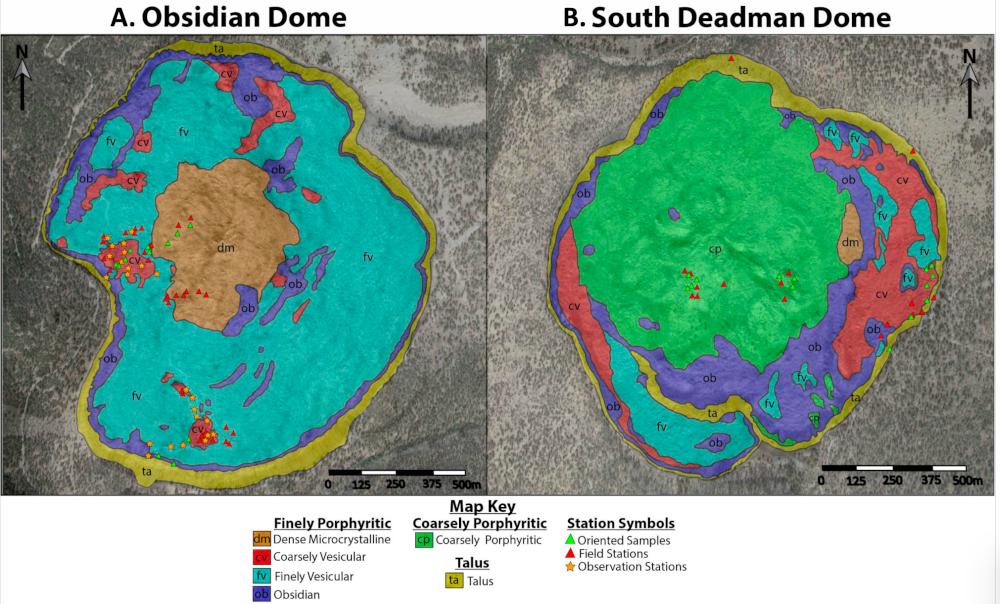
\includegraphics[width=0.95\textwidth]{figs/unitMapping-small.png}
\caption{Textural lithologic distribution maps of lavas for (A) Obsidian dome and (B) South Deadman dome.}
\label{fig:unitMapping}
\end{figure}

\begin{figure}
   \centering
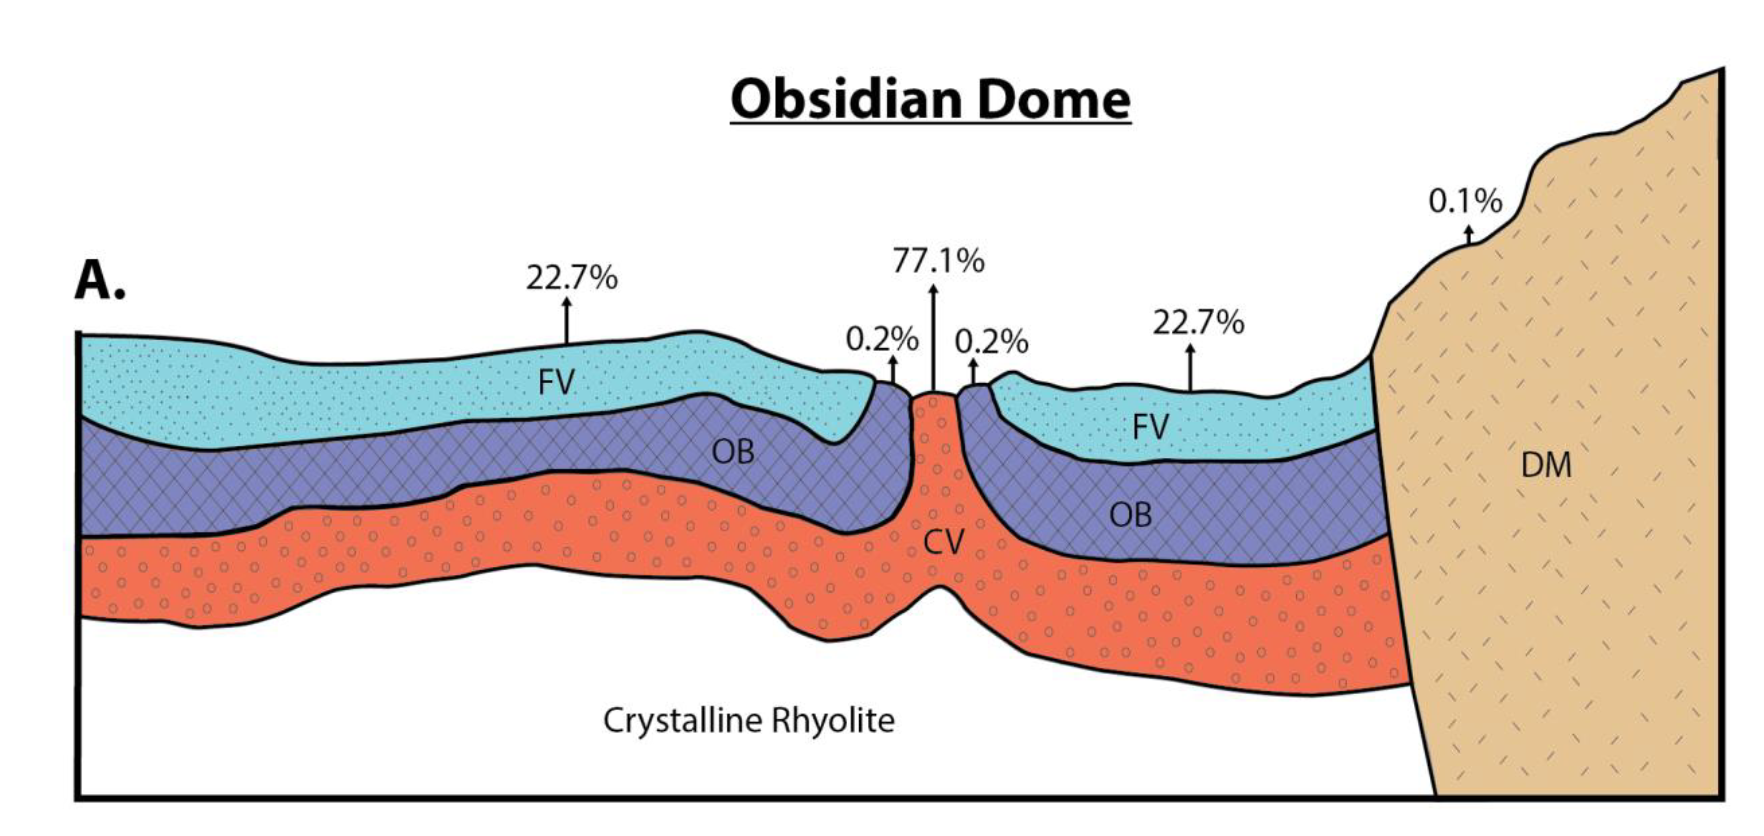
\includegraphics[scale=0.5]{figs/crossSection.png}
\caption{Schematic diagrams depicting total calculated gas flux percentages during the final stages of lava emplacement at Obsidian dome. Total gas flux for each lithologic unit was calculated using the gas flux model of Edmonds et al. (2003), and the gas flux percentages represent the percent gas flux for each lithologic unit relative to the total gas flux calculated for all units, and does not consider additional degassing that occurs through conduit processes, fractures, tuffisite veins, or porous pathways that are too large to measure.}
\label{fig:crossSection}
\end{figure}

\begin{figure}
   \centering
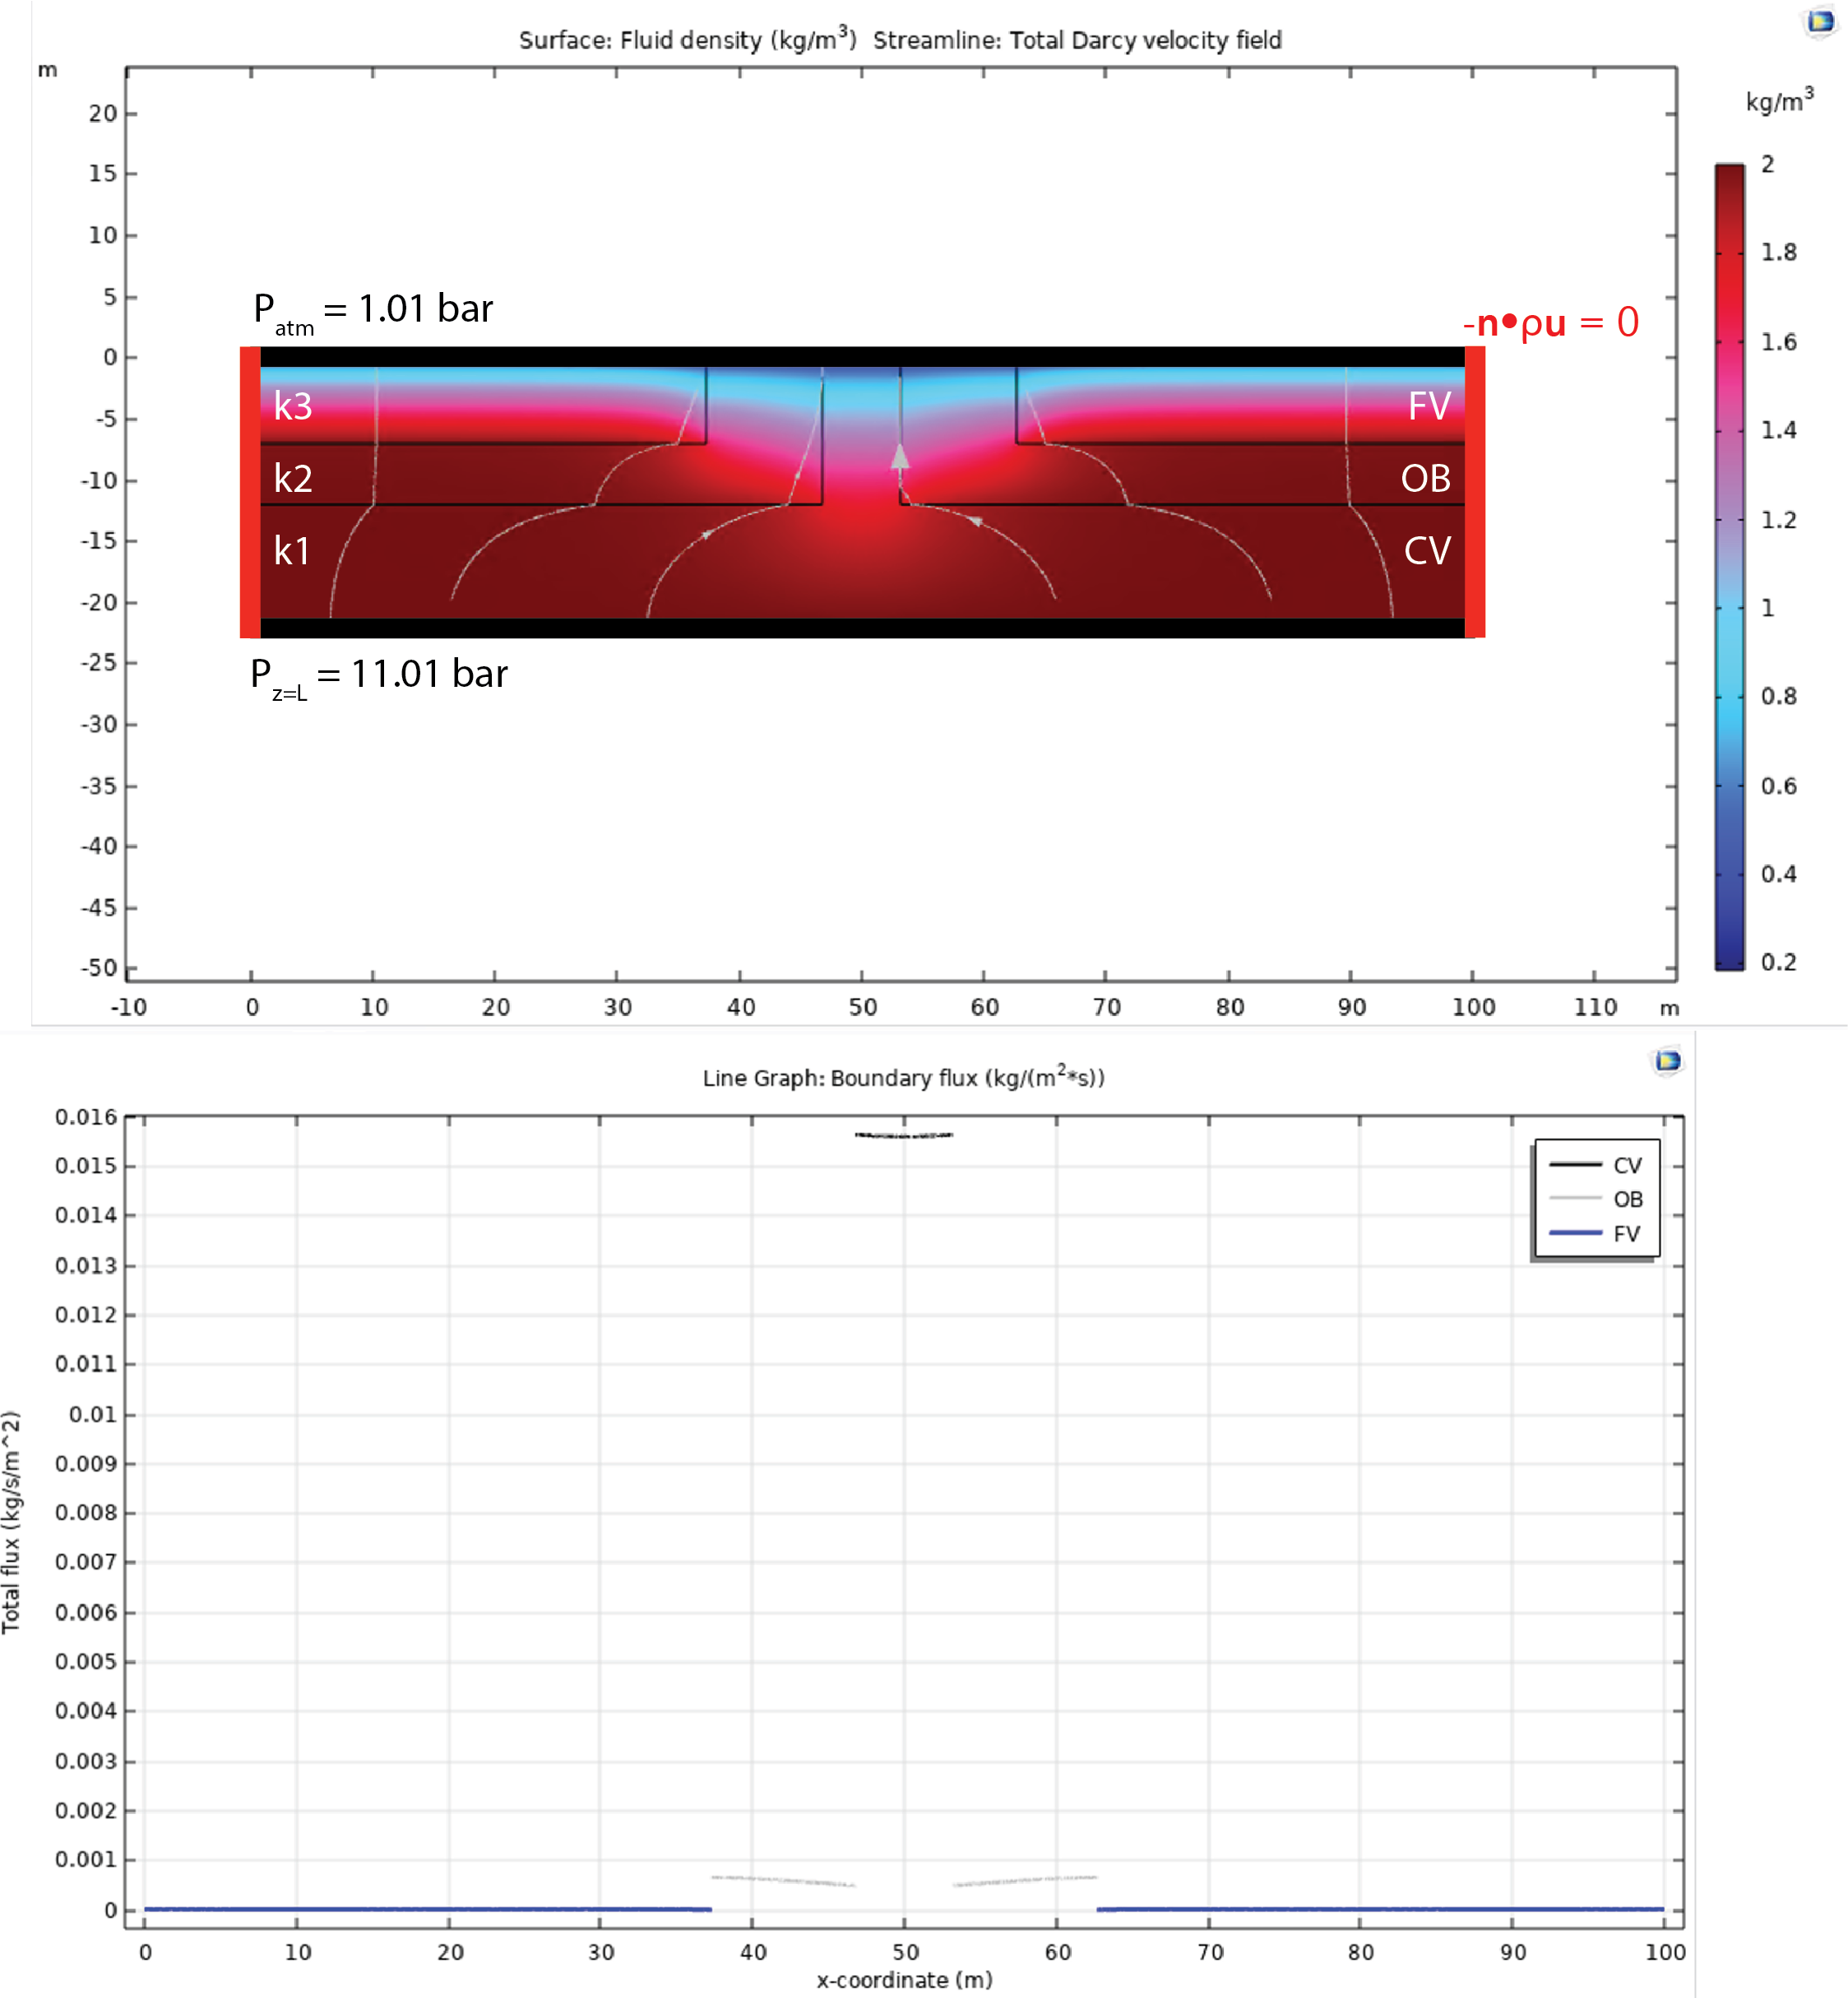
\includegraphics[scale=0.8]{figs/comsolDarcyLaw_units.png}
\caption{Top figure shows gas density in unit layers CV, FV, and OB, with permeabilities k1, k2, and k3, respectively (see Table \ref{tab:UnitPermPoro}). Streamlines indicate the direction of gas flow. Pressure boundary conditions at the base and surface of the units are shown in black, and no flow boundary conditions at the side of the units are shown in red. The bottom figure shows the gas flux at the surface.}
\label{fig:COMSOLresults}
\end{figure}


\begin{table}[h]
\center
      \small
      \begin{tabular}{lllll}
      \hline
      \textbf{Unit} & \textbf{Permeability (m\textsuperscript{2})} & \textbf{Connected porosity (\%)}  & \textbf{Height (m)} & \textbf{Percent of total dome surface area} \\  
      \hline
      CV & 6.87E-12 & 50.0 & 10 & 6.4 \\
      FV & 2.18E-13 & 23.2 &  7 & 74.6 \\
      OB & 4.94E-15 & 3.24 & 5 & 19.0 \\ 
\end{tabular}%}
\caption{Average permeability, porosity, height, and percent of total dome surface area of each textural unit.} 
\label{tab:UnitPermPoro}
\end{table}

\printbibliography

\end{document}
